\section{Linear programs}

\lecture{May 2}
\begin{example}
  Suppose we are selling apples and bananas at a stand.
  Apples sell for \$2 per kilogram, and bananas sell for \$1.5 per kilogram.
  Our stand holds up to 75 kilograms of fruits.
  Also, there are only 4 square metres of shelf space.
  Each kilogram of apples/bananas takes up roughly 0.08/0.05 square metres of shelf space, respectively.
  How much of each fruit should we stock to maximize the total sales?
\end{example}
\begin{sol}
  Let $x_1$, $x_2$ be weight of apples, bananas (kg).
  Define objective function $\max\ 2x_1 + 1.5x_2$.
  Add constraints $x_1 + x_2 \leq 75$ for weight, $0.08x_1 + 0.05x_2 \leq 4$ for shelf space, and $x_1, x_2 \geq 0$ for common sense.

  Summarize as a \term*{linear program}:
  \begin{equation*}
    \begin{aligned}
      \max\                      &  & \multicolumn{2}{l}{$2x_1 + 1.5x_2$}           \\
      \text{subject to (s.t.)}\  &  & x_1 + x_2                           & \leq 75 \\
                                 &  & 0.08x_1 + 0.05x_2                   & \leq 4  \\
                                 &  & x_1, x_2                            & \geq 0
    \end{aligned}
  \end{equation*}

  Trial and error:
  \begin{itemize}[nosep]
    \item $(x_1, x_2) = (30, 20)$ satisfies constraints (\term*{feasible}) with \term*{objective value} 90
    \item $(x_1, x_2) = (31, 20)$ feasible with objective value 92
    \item $(x_1, x_2) = (50, 0)$ feasible with objective value 100
    \item $(x_1, x_2) = (8\frac13, 66\frac23)$ feasible with objective value 116$\frac23$
          (claim without proof that this is \term*{optimal})
  \end{itemize}

  N.B.: we take domain to be $\R$ since we can take fractional parts of a kilogram of fruit

  Plot feasible solutions:
  \begin{center}
    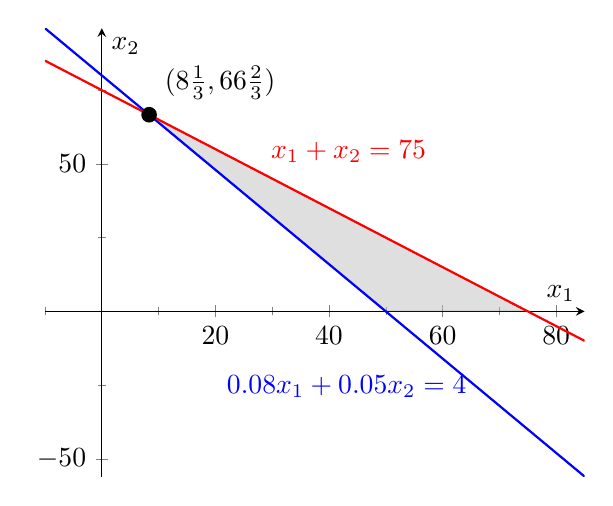
\begin{tikzpicture}
      \begin{axis}[
          axis lines=middle,
          xlabel=$x_1$,
          ylabel=$x_2$,
          minor tick num=1,
        ]
        \addplot[fill=gray!50, opacity=0.5] coordinates {(25/3,200/3) (50,0) (75,0)} -- cycle;
        \addplot[domain=-10:85, blue, thick] {(4-0.08*x)/0.05} node[left, pos=0.8] {$0.08x_1 + 0.05x_2 = 4$};
        \addplot[domain=-10:85, red, thick] {75-x} node[above right, pos=0.4] {$x_1 + x_2 = 75$};
        \node[fill=black, circle, inner sep=2pt, label={above right:$(8\frac13,66\frac23)$}] at (25/3,200/3) {};
      \end{axis}
    \end{tikzpicture}
  \end{center}
  Bound by convex region defined by axes, $x_1 + x_2 = 23$,
  and $0.08x_1 + 0.05x_2 = 4$ to give optimal solution at vertex
\end{sol}

\paragraph{Course overview}
\begin{itemize}[nosep]
  \item Formulation/modelling: create mathematical programs from problems
  \item Solving linear programs: use simplex method to optimize
  \item Geometric interpretation: conceptualize linear programs and simplex method
  \item Integer programs: linear programs defined over $\Z$
  \item Nonlinear programs: convex functions
\end{itemize}

\begin{defn}[optimization problem]
  Given a set of \term{feasible points} $A \subseteq \R^n$ and $f : A \to \R$,
  find some $x \in A$ that minimizes or maximizes the \term{objective value} $f(x)$.

  Composed of \term{decision variables} $\vb x \in \R^n$,
  the \term{objective function} $\max f(\vb x)$ or $\min f(\vb x)$,
  and some \term{constraints} of the form $g_i(\vb x) \leq b_i$
\end{defn}

\begin{defn}[affine function]
  Function of the form $f(\vb x) = \vb a^T \vb x + b = a_1x_1 + \dotsb + a_nx_n + b$ for constants $\vb a$ and $b$
\end{defn}

\begin{defn}[linear function]
  Affine function with $b=0$
\end{defn}

\begin{defn}[linear program]
  An optimization problem with affine objective function $f(\vb x)$ and finitely many linear constraint functions $g_i(x) \geq b_i$ (or $\leq b_i$ or $= b_i$) with constant $\vb b$.

  N.B.: constraints cannot be strict inequalities
\end{defn}

\section{LP Formulation}

\begin{example}
  A company makes 4 types of products, each requiring time on two different machines and two types of labour. The amount of machine time and labour needed to produce one unit of each product along with its sale price are summarized in the following table.
  \begin{center}
    \begin{tabular}{c|ccccc}
      Product & Machine 1 & Machine 2 & Skilled labour & Unskilled labour & Unit sale price \\ \hline
      1       & 11        & 4         & 8              & 7                & 300             \\
      2       & 7         & 6         & 5              & 8                & 260             \\
      3       & 6         & 5         & 5              & 7                & 220             \\
      4       & 5         & 4         & 6              & 4                & 180             \\
    \end{tabular}
  \end{center}
  Each month, the company can use up to 700 hours on machine 1, and 500 hours on machine 2, with no cost. The company can hire up to 600 hours of skilled labour at \$8 per hour, and up to 650 hours of unskilled labour at \$6 per hour. How should the company operate to maximize their monthly profit?
\end{example}
\begin{sol}
  Let $\vb x \in \R^4$ be number of units of products, $y_s$ and $y_u$ be hours of labour hired

  Let the objective function be $\max \enspace 300 x_1 + 260 x_2 + 220 x_3 + 180 x_4 - 8y_s - 6y_u$ (unit sale revenue net of labour costs)

  Let the constraints be $11x_1 + 7x_2 + 6x_3 + 5x_4 \leq 700$ (machine 1), $4x_1 + 6x_2 + 5x_3 + 4x_4 \leq 500$ (machine 2), $8x_1 + 5x_2 + 5x_3 + 6x_4 = y_s$, $7x_1 + 8x_2 + 7x_3 + 4x_4 = y_u$ (defining $y_s$ and $y_u$), $y_s \leq 600$, $y_u \leq 650$ (labour), and $x_1, x_2, x_3, x_4, y_s, y_u \geq 0$ (non-negativity)
\end{sol}

\lecture{May 4}
\begin{example}
  A certain company provides heading oil for the local commnity. They have historical data that helps them predict demand for heating oil in the next four months: 5000, 8000, 9000, 6000 (litres/month)

  At the beginning of each month, they can purchase oil from the supplier at the current market rate. The projected rates are given: 0.75, 0.72, 0.92, 0.90 (\$/litre)

  There is a storage tank that holds up to 4000 litres of oil, and at the start of month 1, it contains 2000 litres. How should the company buy the required oil to minimize the total money spent?
\end{example}
\begin{sol}
  Let $x_i$ be the amount of oil purchased in the $i$th month, and $y_i$ be the amount of oil in the storage tank at the start of month $i$.

  Then, we want to minimize $0.75x_1 + 0.72x_2 + 0.92x_3 + 0.9x_4$.

  The storage tank constrains us by $y_i \leq 4000$ and the problem gives $y_1 = 2000$.

  Non-negativity gives $x_i, y_i \geq 0$.

  For each demand $d_i$, we have $x_i + y_i = d_i + y_{i+1}$.

  Then, we can write:
  \begin{lp}{\min}{0.75x_1 + 0.72x_2 + 0.92x_3 + 0.9x_4}
     &  & y_1, y_2, y_3, y_4              & \leq 4000    \\
     &  & y_1                             & = 2000       \\
     &  & x_1 + y_1                       & = 5000 + y_2 \\
     &  & x_2 + y_2                       & = 8000 + y_3 \\
     &  & x_3 + y_3                       & = 9000 + y_4 \\
     &  & x_4 + y_4                       & = 6000       \\
     &  & x_1,x_2,x_3,x_4,y_1,y_2,y_3,y_4 & \geq 0
  \end{lp}
\end{sol}

\begin{example}
  Instead of minimizing the total money spent, suppose we do not have much money to spend each month, and we want to reduce the maximum amount spent in a month.
\end{example}
\begin{sol}
  Let $M = \max \{0.75x_1, 0.72x_2, 0.92x_3, 0.9x_4\}$.

  Since $M$ is not linear, we cannot simply put $\min M$ in an LP.

  Instead, define $m$ with constraints $m \geq 0.75x_1$, $m \geq 0.72x_2$, $m \geq 0.92x_3$, $m \geq 0.9x_4$.

  Since we are doing $\min m$, we are guaranteed that the optimal solution will give $m = M$ (if $m$ is not $M$, we can make $m$ smaller).
\end{sol}

\begin{example}
  Given a set of data points $\{(x_i, y_i) : i = 1,\dotsc,n\}$ on the plane. Find a line $y = ax + b$ that ``best fits'' this set of data points.
\end{example}
\begin{sol}
  Define ``best fit'' as minimizing total vertical distance between points and the line.

  That is, we must minimize $\sum \abs{ax_i + b - y_i}$, but that is not affine.

  Define instead the errors $e_i$ associated with the point $i$.

  We want to constrain $e_i = \abs{ax_i + b - y_i}$, which we can do with $e_i \geq ax_i + b - y_i$ and $e_i \geq y_i - ax_i - b$ since $\abs{x} = \max\{x, -x\}$.

  Then, we can use $\min \sum e_i$ as above to get the final LP:
  \begin{align*}
    \min \        & \sum e_i                \\
    \text{s.t.}\  & e_i \geq ax_i + b - y_i \\
                  & e_i \geq y_i - ax_i - b
  \end{align*}
  \textbf{N.B.:} since $e_i$, $e_j$ do not share constraints when $i \neq j$, $\min \sum e_i$ is equivalent to $\min e_1, \dotsc, \min e_n$.
\end{sol}

\begin{xca}
  Modify this to find the best fit parabola. Is this an LP?
\end{xca}
\begin{sol}
  Yes, since considering the error function $ax_i^2 + bx_i + c - y_i$ is still linear with respect to the variables for optimization $a$, $b$, and $c$.
\end{sol}

\section{Formulating IPs}

\lecture{May 9}
\begin{example}
  Consider the job application process where a company has 3 positions available, and there are 4 applicants for these jobs. For each applicant and position, the company assigns a number indicating how well the applicant is suited for the position. The goal is to hire a different applicant for each position to maximize the total suitability.

  \[
    M = \begin{pNiceMatrix}[first-row,first-col]
                                            & \Block{1-4}{\text{Candidates}} &   &   &   \\
      \Block{3-1}{\rotate \text{Positions}} & 3                              & 5 & 2 & 4 \\
                                            & 3                              & 1 & 4 & 3 \\
                                            & 1                              & 4 & 2 & 3
    \end{pNiceMatrix}
  \]
\end{example}
\begin{sol}
  Want: For each position, who gets that position

  Define: Create binary variable $x_{ij}$ for each position $i$ and candidates $j$. Let $x_{ij} = 1$ if position $i$ given to candidate $j$, and $0$ otherwise

  Objective function: $\max \sum\sum M_{ij}x_{ij}$

  Constraints: $\sum_{j} x_{ij} = 1$ for each $i$ (each position filled by exactly one candidate), and $\sum_i x_{ij} \leq 1$ for each $j$  (each candidate takes at most one position), $x_{ij} \geq 0$, $x_{ij} \leq 1$, $x_{ij} \in \Z$ (integrality)
  \begin{align*}\max\ & \sum_{i=0}^3\sum_{j=0}^4 M_{ij}x_{ij} \\ \text{s.t.}\ & \sum_{j=0}^4 x_{ij} = 1 & i = 1,\dotsc,3 \\ &\sum_{i=0}^3 x_{ij} \leq 1 & j = 1,\dotsc,4 \\ & 0 \leq x_{ij} \leq 1, x_{ij} \in \Z\end{align*}
\end{sol}

\begin{notation}
  We define $x \in \{0,1\}$ to mean the constraints $0 \leq x \leq 1$ and $x \in \Z$
\end{notation}

\begin{example}[Knapsack problem]
  There are 4 types of items that you can put into your backpack. You can take any integer number of units of any item. However, you can only carry a maximum of 40 pounds. Each unit of item you take is also worth a certain amount of money. The goal is to maximize the total value of the items you carry.
  \begin{center}
    \begin{tabular}{r|cccc}
      Item         & A  & B  & C  & D  \\ \hline
      Weight (lbs) & 1  & 7  & 3  & 2  \\
      Value (\$)   & 10 & 50 & 20 & 15 \\
    \end{tabular}
  \end{center}
\end{example}
\begin{sol}
  Let $x_i$, $i = A,B,C,D$ be the number of units of $i$ packed

  Objective function: $\max 10x_A + 50x_B + 20x_C + 15x_D$

  Constraints: $x_A + 7x_B + 3x_C + 2x_D \leq 40$ (weight limit), $x_i \geq 0$, $x_i \in \Z$ (integrality)

  \[
    \begin{aligned}
      \max\         &  & 10x_A + 50x_B + 20x_C + 15x_D           \\
      \text{s.t.}\  &  & x_A + 7x_B + 3x_C + 2x_D      & \leq 40 \\
                    &  & x_A,x_B,x_C,x_D               & \geq 0  \\
                    &  & x_A,x_B,x_C,x_D               & \in \Z
    \end{aligned}
  \]
\end{sol}

\begin{example}
  Suppose we are allowed to take A only if we take at least one unit of B.
\end{example}
\begin{sol}
  Want: if $x_B = 0$, then we must have $x_A = 0$. If $x_B \geq 1$, no restriction on $A$.

  Equivalently, add the constraint $x_A \leq x_B \max x_A = 40x_B$. When $x_B = 0$, the RHS goes to $0$ and constrains $x_A = 0$. Otherwise, since $x_B \geq 1$, $40x_B \geq 40$ which is the maximum value of $x_A$, so there are effectively no constraints on $x_A$.
\end{sol}

\begin{example}
  Suppose we want the following conditions to hold:
  \begin{enumerate}[1.,nosep]
    \item We carry at least 5 units of items A and/or B; or
    \item We carry at least 7 units of items C and/or D.
  \end{enumerate}
\end{example}
\begin{sol}
  Define a binary variable $y$. Want: $y = \begin{cases*}1&condition 1 is true\\0&condition 2 is true\end{cases*}$

  If $y = 1$, then $x_A + x_B \geq 5$; if $y = 0$, no restrictions on $x_A$, $x_B$. We can implement this by adding the constraint $x_A + x_B \geq 5y$, since $y = 0$ will send the RHS to $0$

  If $y = 0$, then $x_C + x_D \geq 7$; if $y = 1$, no restrictions on $x_C$, $x_D$. Similarly implement with $x_C + x_D \geq 7(1-y)$, since $y=1$ will send the RHS to $0$

  Notice that setting $y$ does not force the other condition \emph{not} to hold, i.e., this implements an inclusive or.

  In summary: $x_A + x_B \geq 5y$, $x_C + x_D \geq 7(1-y)$, and $y \in \{0,1\}$

  \textbf{N.B.:} When feeding these constraints into an algorithm, ensure that the constraints are truly linear, i.e., move variables to one side. For example, $x_A + x_B - 5y \geq 0$
\end{sol}

\begin{xca}
  Implement an exclusive or of these two conditions
\end{xca}

\begin{example}
  Suppose that the value of item A is \$10 for the first 5 units, but any more units beyond that has value \$5.
\end{example}
\begin{sol}
  Separate $x_A$ into two variables $x_{A1}$ for first five units and $x_{A2}$ for remainder.
  Then, we have $x_A=x_{A1}+x_{A2}$ and change the objective function to $10x_{A1} + 5x_{A2} + 50x_B + 20x_C + 15x_C$.

  We can create a constraint to force $x_{A2}$ only to go up when $x_{A1}$ is 5 with $x_{A2} \leq (x_{A1} - 4)\max x_{A2}$ which will work in tandem with the non-negativity constraint. This is not actually necessary since the maximum will always fill $x_{A1}$ before $x_{A2}$ because it is worth more (i.e. trading one $x_{A2}$ for $x_{A1}$ will increase the objective function by 5)

  In summary: change the objective function and add the constraints $x_A = x_{A1} + x_{A2}$, $x_{A1} \leq 5$, $x_{A1},x_{A2} \geq 0$, $x_{A1}, x_{A2} \in \Z$
\end{sol}

\lecture{May 11}
\begin{notation}[vector notation]
  Write $\mathbb{1} := (1,\dotsc,1)^T$ and $x \leq y$ if $x_i \leq y_i$ for all $i$.
\end{notation}

\begin{defn}[graph]
  $G = (V, E)$ consists of a set of objects $V$ (\term{vertices}) and a set of unordered pairs of vertices $E$ (\term{edges}).

  We restrict graphs by disallowing empty graphs, redundant edges, directed edges, or self-connections.
\end{defn}

\begin{example}\label{ex:graph}
  $G = (V, E)$ by $V = \{1,2,3,4\}$, $E=\{12,23,34,41,24\}$
  \begin{center}
    \tikz\graph{{1,4}--{2,3}; 1--4; 2--3; 2--4};
  \end{center}
\end{example}

\begin{defn}[incidence relation]
  For an edge $e=uv$, $e$ is incident to $u$ and $v$.
  $\delta(v)$ is the set of all edges incident to $v$.

  The \term{incidence matrix} $B \in \{0,1\}^{\abs{V}\times\abs{E}}$
  has rows indexed by $V$, columns by $E$, and $B_{ve} = 1$
  when $e \in \delta(v)$ and $0$ otherwise.
\end{defn}
\begin{example}
  For \cref{ex:graph}, $B = \begin{pNiceMatrix}[first-row,first-col]
        & e_1 & e_2 & e_3 & e_4 & e_5 \\
      1 & 1   & 0   & 0   & 1   & 0   \\
      2 & 1   & 1   & 0   & 0   & 1   \\
      3 & 0   & 1   & 1   & 0   & 0   \\
      4 & 0   & 0   & 1   & 1   & 1
    \end{pNiceMatrix}$.
\end{example}
\begin{remark}
  Each column has exactly two ones, so $B\mathbb{1} = 2\mathbb{1}$.
\end{remark}

\begin{defn}[matching]
  $M \subseteq E$ where each vertex is incident with exactly zero or one edge in $M$ (i.e., $\abs{M \cap \delta(v)} \leq 1$ for all $v \in V$)
\end{defn}
\begin{example}
  For \cref{ex:graph}, $\{e_1, e_3\}$ and $\{e_5\}$ are matchings but $\{e_1, e_5\}$ is not since $2$ is incident to both edges
\end{example}

\begin{example}[maximum-weight matching]
  Given graph $G = (V, E)$ and weights $w_e$ for each $e \in E$. Find a matching in $G$ with the maximum edge weight, i.e., maximize $\sum_{e \in M} w_e$.
\end{example}
\begin{sol}
  Define a vector $x \in \{0,1\}^{\abs{E}}$ by $x_e = 1$ if $e \in M$ and $0$ otherwise.
  Then, the objective function is $\max w^T x$.
  To ensure each node appears only once, add constraints $\sum_{e \in \delta(v)} x_e \leq 1$ for each $v \in V$. This is equivalent to taking the incidence matrix $A$ and saying $Ax \leq \mathbb{1}$
  This gives us the integer program
  \begin{align*}
    \max\         & w^T x                         \\
    \text{s.t.}\  & Ax \leq \mathbb{1}            \\
                  & x_e \in \{0,1\} \quad e \in E
  \end{align*}
\end{sol}

\begin{defn}[$v_1$,$v_k$-path]
  Sequence of edges $v_1v_2, v_2v_3, \dotsc, v_{k-1}v_k$ such that $v_1,\dotsc,v_k$ are distinct
\end{defn}
\begin{example}\label{ex:path}
  Consider graph $(\{s,t,a,b,c,d\}, \{sa,sc,ab,ac,bd,bt,cb,cd,dt\})$.
  \begin{center}
    \begin{tikzpicture}
      \graph[math nodes]{s--{a--b,c--d}--t; a--c; b--d; c--b};
    \end{tikzpicture}
  \end{center}  
  Then, $sa,ab,bt$ and $sc,cb,bd,dt$ are $s$,$t$-paths but $sa,ab,bc,cd,cb,bt$ is not since $b$ is visited twice.
\end{example}

\lecture{May 16}

\begin{problem}[shortest path]
  Given graph $G = (V, E)$, vertices $s$ and $t$, and positive weights $w_e$ for each $e \in E$. Find an $s$,$t$-path $P$ with the minimum edge weight, i.e., minimize $\sum_{e \in P} w_e$.
\end{problem}

Define a vector $x \in \{0,1\}^{\abs{E}}$ by $x_e = 1$ if $e \in P$ and $0$ otherwise.

The objective function is $\min w^T x$.

Need to constrain $x$ into a path: use cuts.

\begin{defn}[cut]
  The \term*{cut induced by vertices $W$} is the set $\delta(W)$ of all edges with exactly one endpoint in $W$.
  Formally, $\delta(W) = \{uv \in E : u \in W, v \not\in W\}$.

  An \term{$s,t$-cut} $\delta(W)$ has $s \in W$ and $t \not\in W$.
\end{defn}
\begin{example}
  In \cref{ex:path}, $W=\{s,a,b\}$ induces the cut $\delta(W) = \{sc,ac,bc,bd,bt\}$
  \begin{center}
    \begin{tikzpicture}
      \graph[math nodes,simple]{s--{a--b,c--d}--t; s--[red]c; a--[red]c; b--[red]d; b--[red]c; b--[red]t};
    \end{tikzpicture}
  \end{center}
\end{example}

\begin{prop}
  Notice that the edges in an $s,t$-cut separate $s$ from $t$, so an $s,t$-path must use at least one edge from every $s,t$-cut (formal proof in graph theory course)
\end{prop}

We get a constraint $\sum_{e \in \delta(W)} x_e \geq 1$ for all $s,t$-cuts $\delta(W)$ (that is, for all $W \subset V$ with $s \in W$ and $t\not\in W$)

\begin{prop}
  If a set of edges intersects every $s,t$-cut, then it contains an $s,t$-path
\end{prop}

Minimizing the edge weights will ensure that the extraneous edges are optimized away and the $s,t$-path remains so long as the edge weights are all positive.

This gives us a final IP of
\begin{align*}
  \min\         & w^T x                                                               \\
  \text{s.t.}\  & \sum_{e \in \delta(W)} x_e \geq 1 & \text{$\delta(W)$ an $s,t$-cut} \\
                & x_e \geq 0, x_e \in \Z            & e \in E
\end{align*}

\section{Formulating NLPs}

\begin{defn}[non-linear program]
  A program of the general form $\min f(x)$ subject to $g_i(x) \leq 0$ for some arbitrary functions $f : \R^n \to \R$, $g_i : \R^n \to \R$ with no restrictions
\end{defn}
\begin{example}
  Among all the points $x$ that satisfy $Ax \leq b$, find one that is closest to the target point $\bar x$
\end{example}
\begin{sol}
  We can take the norm and minimize $\norm{x - \bar x} = \sqrt{\sum(x_i-\bar x_i)^2}$.
  This gives us the non-linear program $\min \norm{x - \bar x}, \text{s.t.\ } Ax \leq b$.
\end{sol}

\lecture{May 18}
Since the definition for NLP has no constraints on $f$ and $g_i$, a LP is an NLP.

The integrality constraint makes IPs not NLPs.
To get around this, use a periodic function like $\sin \theta = 0$ which permits values $\theta = k\pi$ for integer $k$, so $x \in \Z \Harr \sin x\pi  = 0$.
Using this makes IPs into NLPs.

If we can solve NLPs, we can also solve LPs and IPs.

\section{LP outcomes}

An algorithm that solves LPs should produce:
\begin{itemize}[nosep]
  \item The optimal solution (or that no solution exists)
  \item Certificate of correctness that reduces complexity of verification
\end{itemize}

\begin{defn}[infeasibility]
  No feasible solutions exist.
\end{defn}

\begin{example}
  $\max x$ s.t. $x \leq 2$ and $x \geq 3$. Obviously, no $x$ exists.
\end{example}

\begin{example}
  $\max{(3,1,-7,4)x}$ s.t. $\mqty(-5&4&3&-1\\2&1&-5&3\\-1&-3&1&-2)x = \mqty(3\\-2\\1)$ and $x \geq \mathbb{0}$.

  Taking $-2R_1 - 3R_2 - 4R_3$, we get $8x_1+x_2+5x_3+x_4 = -4$ but each entry in $x$ must be non-negative, so this is impossible.

  Formally, we can let $y = (-2,-3,-4)^T$, then multiply on the left by $y^T$ to give us the same equation as $(8,1,5,1)x = -4$.

  Then, $y$ is the \term{certificate of infeasibility}.
\end{example}

\begin{prop}
  The system $Ax = b$, $x \geq \mathbb{0}$ is infeasible if there exists a vector $y$ such that $y^T A \geq \mathbb{0}$ but $y^T b < 0$
\end{prop}
\begin{prf}
  Suppose the system is feasible with $x$ as the feasible solution. Then, $Ax = b$ and $x \geq \mathbb{0}$. However, $y^T A x \geq 0$ and $y^T b < 0$. Contradiction.
\end{prf}

The converse is also true. Proof will come later as Farkas' Lemma.

\begin{defn}[unboundedness]
  Infinitely better feasible solutions exist.

  Formally, a max (resp. min) LP is \term*{unbounded} if there exists a series of feasible solutions $x(t)$ with the objective value of $x(t)$ approaching $+\infty$ (resp. $-\infty$) as $t \to \infty$.
\end{defn}
\begin{example}
  $\max x$ s.t. $x \geq 1$: there is no best solution (cf. strict inequalities)
\end{example}
\begin{example}
  $\max{} (-1,2,-3,4)x$ s.t. $\mqty(3&0&2&-5\\-2&3&-4&4)x=\mqty(4\\1)$ and $x \geq \mathbb 0$.

  Consider $\bar x = (3,1,0,1)^T$ and $d = (0,4,5,2)^T$. Define $x(t) = \bar x + td$ and consider $t$ from $0 \to \infty$.
  We must show feasibility and unboundedness.

  Obviously, $x(t) \geq \mathbb 0$ since $\bar x, d \geq \mathbb 0$ and $t \geq 0$.

  Notice $Ax(t) = A\bar x + tAd = (4,1)^T + t(0,0)^T = b$. That is, $\bar x$ solves $Ax = b$ and $d$ lies in the kernel of $A$.

  The objective value $c^T x(t) = c^T(\bar x + td) = c^T\bar x + tc^T d = 3 + t$ clearly goes to $+\infty$ as $t \to \infty$.

  Then, $(\bar x, d)$ is a certificate of unboundedness for the LP.
\end{example}

\begin{prop}
  The LP $\max \{c^T x : Ax=b, x \geq \mathbb 0\}$ is unbounded if there exist vectors $\bar x$ and $d$ such that $\bar x, d \geq \mathbb 0$, $Ad = \mathbb 0$, $c^T d > 0$.
\end{prop}
